
\chapterbegin{Servidor}
\label{chp:App}
\minitoc

\sectionx{Introducci�n}
\begin{wrapfigure}{L}{0.4\textwidth}
	\begin{center}
		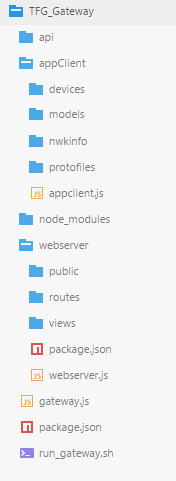
\includegraphics[width=0.3\textwidth]{graphs/estructuraServidor.png}
	\end{center}
	\caption{Estructura del directorio del servidor}
	\label{fig:estructuraServidor}
\end{wrapfigure}

El servidor se puede dividir en dos partes \textit{Front-end} y \textit{Back-End} que son t�rminos que se refieren a la separaci�n entre una capa de presentaci�n y una capa de acceso a datos respectivamente. 

\sectionx{Estructura del servidor}

El servidor est� compuesto por el directorio que se observa en la figura \ref{fig:estructuraServidor} y a continuaci�n se describe la funci�n de cada directorio:


\begin{description}
	\item[api: ] en este directorio se encuentran las definiciones de llamadas REST al servidor.
	\item[appClient: ] Esta carpeta contiene el \textit{Back-end} de la web:
	\begin{description}
		\item[devices: ] se definen las funciones relacionadas con la gesti�n de los nodos.
		\item[models: ] aqu� se definen los modelos para guardarlos en la base de datos.
		\item[nwkinfo: ] se definen las funciones relacionadas con la gesti�n del concentrador.
		\item[protofiles: ] aqu� se almacenan los ficheros .proto de \textit{Protocol Buffers}.
		\item[appClient.js: ] en este fichero se inicia el servidor que se comunica con el concentrador y se procesan los mensajes.
	\end{description}
	\item[node\_modules: ] librer�as utilizadas en el proyecto.
	\item[webserver: ] en este directorio est� contenida la l�gica del \textit{Front-end}:
	\begin{description}
		\item[public: ] interfaz del cliente en AngularJS.
		\item[routes: ] Definici�n de rutas.
		\item[views: ] archivos html de las vistas.
		\item[webserver.js: ] se inicia el cliente y se gestiona las peticiones a la web por parte del usuario.
	\end{description}
	\item[gateway.js: ] inicia el \textit{back-end} y el \textit{front-end} y la comunicaci�n entre ambas por \textit{web-sockets}.
	\item[run\_gateway.sh: ] \textit{script} para iniciar el servidor.
\end{description}

\sectionx{Back-end}

El \textit{Back-end} es el �rea que se dedica a la l�gica, en este encontramos una interfaz que se encarga de comunicarse con el concentrador y otra que se encarga de comunicarse con el \textit{Front-end} usando \textit{Web-Sockets}.


Al inicio del archivo \textit{appClient.js} se abre el puerto 3000 y se mantiene a la escucha hasta que el concentrador se conecta. Cuando el concentrador se conecta, este el env�a la informaci�n de configuraci�n. \\

Toda la informaci�n de la red se almacena en una base de datos MongoDB\R, tambi�n se almacena los datos enviados por los nodos as� como sus par�metros de configuraci�n.\\

Una vez la conexi�n entre el concentrador y el \textit{back-end} se ha establecido, ambos se quedan a la espera de que el usuario desde el \textit{front-end} permita la conexi�n de los nodos a la red.


\sectionx{Front-end}

El \textit{Front-end} es la interfaz del servidor con el usuario. Para facilitar el control de las vistas se ha utilizado el \textit{framework AngularJS}.\\

Angular es un \textit{framework} \ac{MVC} para la construcci�n de aplicaciones de una �nica p�gina del lado del cliente en HTML y JavaScript.\\

Como se ha mencionado anteriormente, el patr�n que se usa en Angular es el conocido como Modelo, Vista y Controlador:

\begin{description}
	\item[Vistas: ] Ser� el c�digo HTML y todo lo que presente los datos o informaci�n.
	\item[Controladores: ] Se encarga de toda la l�gica de la aplicaci�n.
	\item[Modelo: ] El modelo es la estructura que define un tipo de dato, y permite acceder a �l en la base de datos.
\end{description}




\chapterend{}